\section{Statistical methods}\label{appA}

This appendix collects the estimator definitions used in the main text. CoEval reports the agreement of the judge
panel using intraclass correlation. For an average-measures design over \(k\) judges, the ICC(3,k) reliability is

\[\mathrm{ICC}(3,k) \;=\; \frac{MSR - MSE}{MSR},\]

where \(MSR\) is the between-targets (rows) mean square and \(MSE\) the residual mean square. The gain from aggregating
more judges follows the \textbf{Spearman--Brown} prophecy relation: if \(\bar{r}\) is the mean pairwise
inter-judge correlation, the reliability of a \(k\)-judge mean is

\[R_k \;=\; \frac{k\,\bar{r}}{1 + (k-1)\,\bar{r}}.\]

For categorical agreement (e.g., pass/fail rubric criteria) CoEval reports Cohen\textquotesingle s \(\kappa\),

\[\kappa \;=\; \frac{p_o - p_e}{1 - p_e},\]

where \(p_o\) is observed agreement and \(p_e\) the agreement expected by chance. To quantify residual bias and its
uncertainty, CoEval computes the Pearson correlation between a candidate confound (e.g., response length) and the
assigned score, with a \textbf{nonparametric bootstrap} confidence interval: the per-item (length, score)
pairs are resampled with replacement \(B\) times, the correlation is recomputed on each resample, and the
\(2.5\)th--\(97.5\)th percentiles of the bootstrap distribution form the reported 95\% CI. A CI that includes zero
indicates that the corresponding bias is statistically indistinguishable from absent. Across the family of correlation
tests reported in Section~5 we control the false-discovery rate with the Benjamini--Hochberg procedure
(\(\alpha = 0.05\)), and confidence intervals use a \emph{datapoint-clustered} resample wherever observations are
nested (multiple student responses per item).

\section{Rubric structure}\label{appB}

CoEval generates a scoring rubric automatically per task. We examine whether these rubrics are appropriately
task-specialized while sharing a common quality core. Across the four tasks, the 22 auto-generated rubric criteria
exhibit a mean \emph{within-task} semantic similarity of \(0.342\), exceeding the mean \emph{cross-task} similarity
of \(0.294\): criteria cluster by task, as desired. At the same time, a shared universal
\emph{``completeness''} dimension recurs across three of the four tasks, indicating a common quality core.
CoEval\textquotesingle s rubrics are thus specialized to each task\textquotesingle s demands yet anchored by a transferable notion of answer quality.

\begin{figure}[tbp]
\centering
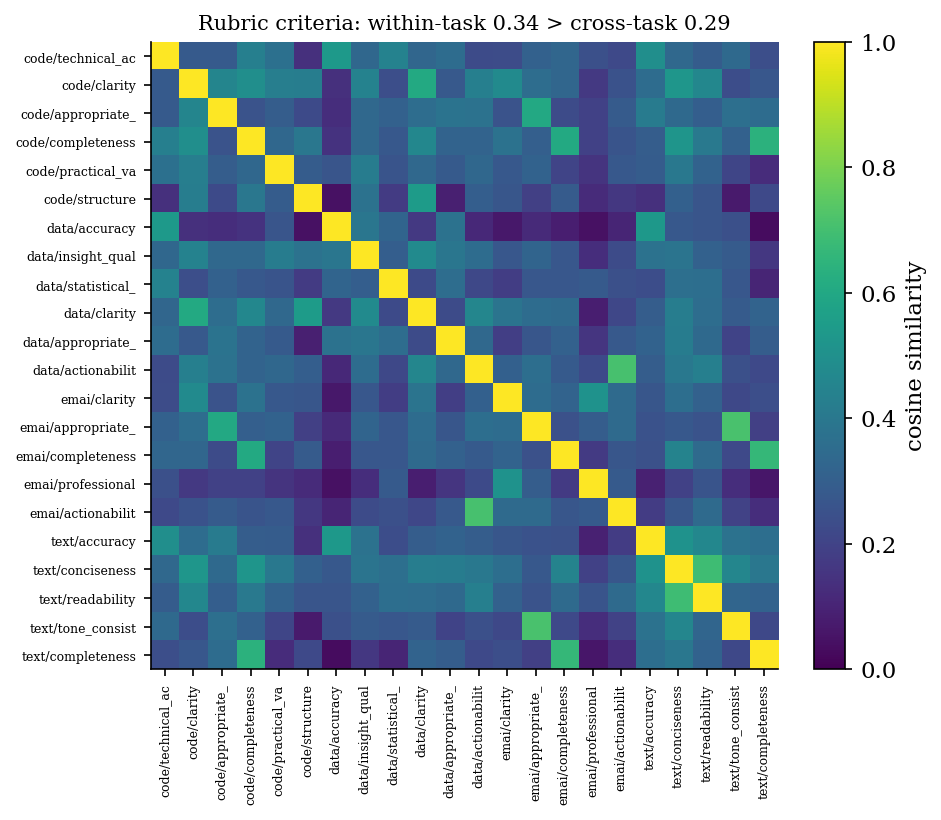
\includegraphics[width=\linewidth]{figures/f5_rubric_heatmap.png}
\caption{\textbf{Figure 3.} Pairwise semantic similarity of the 22 auto-generated rubric criteria across
four tasks. Block structure along the diagonal reflects task specialization (within-task 0.342 \textgreater{} cross-task
0.294), while a recurring ``completeness'' dimension forms a cross-task cluster.}
\end{figure}

\section{Worked examples on data-scarce domains}\label{appC}

The three verticals of Section~5.4 are domains where a practitioner typically has \emph{no} labeled
benchmark and no trustworthy public one: drug--drug interaction (DDI) reasoning, clinical decision support, and
legal analysis. The artifacts below are the \emph{actual} output CoEval generated for each, from a single one-line
task description and with no human labels. From that description the teacher inferred the attribute strata, synthesized
\(40\) contamination-free items stratified over them, and wrote a scoring rubric; the vendor-disjoint panel
(OpenAI~+~Anthropic~+~Google) then ranked three candidate models (Table~G1).

The pipeline is four templated calls to the teacher, all instantiated from the one-line
\texttt{task\_description} (and an optional \texttt{output\_description}). The first two build the attribute
space the items are stratified over; the third writes the rubric the panel scores against; the fourth generates one
contamination-free item per sampled attribute cell. The templates below are the verbatim framework prompts; a sampled
cell such as \emph{severity~=~moderate, mechanism~=~pharmacokinetic, patient\_context~=~pregnancy}
is what binds \texttt{\{target\_attributes\}} and yields the corresponding DDI item shown after Table~C1.

\textbf{(1) Target-attribute map.} Define the axes the benchmark varies over.

\begin{Verbatim}[breaklines=true,breakanywhere=true,fontsize=\small]
Generate synthetic data specifications for the {task_description} task by defining an
attribute space that characterizes possible outputs. Return a JSON object mapping each
attribute name to a list of possible values, and output only the JSON.
\end{Verbatim}


\textbf{(2) Nuance map.} Add surface-variation axes that change phrasing without changing the answer.

\begin{Verbatim}[breaklines=true,breakanywhere=true,fontsize=\small]
Define synthetic data specifications for the {task_description} task by creating a nuanced
variability-focused attribute space. Include only attributes that change document phrasing,
structure, noise, and context, without changing the underlying outputs. Return a single JSON
object mapping each attribute name to a list of allowed values, and output only the JSON.
\end{Verbatim}


\textbf{(3) Auto-rubric.} Write the task-specific scoring factors the judges apply.

\begin{Verbatim}[breaklines=true,breakanywhere=true,fontsize=\small]
For the task {task_description}, where the model's output is {output_description}, create an
evaluation rubric. Return only a JSON object where each key is a quality factor, and each
value is a concise description of that factor. Output only the JSON.
\end{Verbatim}


\textbf{(4) Item synthesis.} Generate one realistic item for a sampled attribute cell.

\begin{Verbatim}[breaklines=true,breakanywhere=true,fontsize=\small]
Generate a realistic benchmark data point.
Task: {task_description}
Output format: {output_description}
Required attributes: {target_attributes}
Nuance: {nuanced_attributes}

Return only a JSON object with exactly two string keys:
  "prompt":   a realistic input text for the task
  "response": the expected output for that input
Output only the JSON. No explanation or markdown.
\end{Verbatim}


Running this pipeline on the three one-line seeds below produces the auto-generated attribute strata and rubrics in
Table~C1, and the verbatim items that follow it.

\begin{table*}[t]
\centering
\small\setlength{\tabcolsep}{4pt}%
\caption{\textbf{Table C1.} From a one-line description to a scored benchmark, for three domains with no
public labeled data. The attribute strata and rubric criteria are auto-generated by the teacher; each domain yields
40 stratified, contamination-free items, scored by the cross-family panel.}
\setlength{\tabcolsep}{4pt}
\begin{tabularx}{\textwidth}{>{\hsize=1.214\hsize\raggedright\arraybackslash}X >{\hsize=1.193\hsize\raggedright\arraybackslash}X >{\hsize=0.593\hsize\raggedright\arraybackslash}X}
\toprule
Domain and one-line seed & Auto-generated attribute strata & Auto-generated rubric \\
\midrule
\textbf{Drug--drug interaction reasoning}\newline 
\emph{"given two or more co-administered drugs and a patient context, assess the interaction, its mechanism, severity, and clinical action"} & severity \{contraindicated, major, moderate, minor\}; mechanism \{pharmacokinetic, pharmacodynamic\};
patient\_\allowbreak{}context \{renal, hepatic, polypharmacy-elderly, pregnancy\} & interaction\_\allowbreak{}accuracy, severity\_\allowbreak{}correct, safety, completeness \\
\textbf{Clinical reasoning}\newline 
\emph{"a clinical reasoning question a clinician would face, requiring medical knowledge and safe, accurate reasoning"} & specialty \{cardiology, infectious\_\allowbreak{}disease, pediatrics, oncology, emergency\}; difficulty \{routine, intermediate, hard\} & clinical\_\allowbreak{}accuracy, safety, completeness, clarity \\
\textbf{Legal analysis}\newline 
\emph{"a legal analysis question requiring identification of the relevant rule and correct application to the facts"} & area\_\allowbreak{}of\_\allowbreak{}law \{contracts, torts, criminal, constitutional, intellectual\_\allowbreak{}property\}; complexity \{basic, intermediate, advanced\} & legal\_\allowbreak{}accuracy, reasoning\_\allowbreak{}quality, completeness, clarity \\
\bottomrule
\end{tabularx}
\end{table*}

One representative \emph{generated} item per domain (verbatim teacher output, labeled with its sampled attribute
cell), showing the synthesized items are specific and realistic rather than templated:

\begin{itemize}
\tightlist
\item
  \textbf{DDI} (severity = moderate, mechanism = pharmacokinetic, patient\_context = pregnancy):
  \emph{"A 30-year-old pregnant woman is prescribed lamotrigine for bipolar disorder and is also taking oral
  contraceptives. Assess the drug--drug interaction between these medications, identify the mechanism, and provide
  the severity and clinical recommendation."}
\item
  \textbf{Clinical} (specialty = cardiology, difficulty = routine):
  \emph{"A 62-year-old male with a history of hypertension and hyperlipidemia presents with progressive shortness of
  breath and occasional palpitations. On examination, you note elevated jugular venous pressure and a third heart
  sound. An ECG shows left ventricular hypertrophy. What is the most likely diagnosis and what initial management
  strategy should be considered?"}
\item
  \textbf{Legal} (area\_of\_law = torts, complexity = basic):
  \emph{"Alice, while jogging in the park, trips over a tree root that has been exposed due to erosion and falls,
  breaking her wrist. The park is owned by the city, and Alice claims the city is liable for her injuries due to
  negligence. Identify the relevant rule and determine if Alice can successfully hold the city liable."}
\end{itemize}

Each item is scored on its rubric by the panel, producing the rankings in Table~G1. On DDI the three judges are
unanimous, \texttt{gpt-4o-mini} (\(0.770\)) \textgreater{} \texttt{gpt-3.5-turbo} (\(0.682\)) \textgreater{}
\texttt{llama-3.2-3b} (\(0.497\)), with non-overlapping confidence intervals; on clinical reasoning the two stronger
models are statistically close (\(0.873\) vs \(0.864\)), which the overlapping intervals correctly expose. The entire path
from a one-line description to a defensible, contamination-free ranking is a single configuration file with no labeled
data and no human raters.

\section{Rankings are domain-specific: why a generic leaderboard misleads}\label{appD}

The case studies above rank models \emph{within} one domain. The premise of a custom-evaluation tool is that this
is necessary: the best model for one domain need not be the best for another, so a single public leaderboard, which
pools tasks into one number, can send a practitioner to the wrong model. We test this directly. From four one-line
descriptions, \emph{math word problems}, \emph{code explanation}, \emph{clinical reasoning}, and \emph{legal
analysis}, CoEval generated \(25\) contamination-free items each (\(100\) items), six candidate models answered them,
and the same vendor-disjoint cross-family panel (OpenAI~+~Anthropic~+~Google) scored every
response: \(1{,}800\) evaluations at full coverage, from one configuration file.

The four per-domain rankings \textbf{disagree sharply}. Three different models take first place across the four
domains, and each winner is stable under a bootstrap over items (\(B=2000\)): \texttt{gpt-4o-mini} tops clinical
reasoning (top with probability \(0.88\)) and code explanation (\(0.60\)), \texttt{gemini-flash} tops legal analysis
(\(1.00\)), and \texttt{claude-3.5-haiku} tops math word problems (\(0.85\)). The movement is not confined to the lead:
\texttt{gpt-4o-mini} falls from first on clinical reasoning to fifth of six on math (where it is top in only
\(0.001\) of bootstrap draws), and \texttt{claude-3.5-haiku} moves the opposite way, from first on math to fifth on
code (Table~D1). The mean cross-domain rank agreement is low (Kendall~\(\tau = 0.19\) averaged over the six
domain pairs); the least-aligned pair, code explanation versus math word problems, has a negative point estimate
(\(\tau = -0.41\)).

This is exactly the regret a generic leaderboard incurs. Pooling the four domains into one average ranks
\texttt{gemini-flash} first, but that model is the correct pick for only one of the four domains (legal analysis);
on clinical reasoning and code explanation the best model is \texttt{gpt-4o-mini}, and on math it is
\texttt{claude-3.5-haiku}, which the pooled board ranks only third. A practitioner who reads the generic
leaderboard and deploys its top model is choosing the domain-best model in just one of four cases. CoEval removes the
guess: it ranks the candidates on the practitioner\textquotesingle s own domain, contamination-free, with no labeled data.

\begin{table*}[t]
\centering
\small\setlength{\tabcolsep}{4pt}%
\caption{\textbf{Table D1.} The same six candidate models ranked by the same cross-family panel on four
CoEval-generated domains diverge: each cell is the model\textquotesingle s rank (1 = best) in that domain, rows ordered by the
generic pooled leaderboard. Three distinct models win the four domains (highlighted), and the pooled-best model
(\texttt{gemini-\allowbreak{}flash}) is domain-best in only one. \texttt{gpt-\allowbreak{}4o-\allowbreak{}mini} swings from 1st to 5th and
\texttt{claude-\allowbreak{}3.5-\allowbreak{}haiku} from 5th to 1st across domains.}
\small
\setlength{\tabcolsep}{4pt}
\begin{tabularx}{\textwidth}{>{\hsize=1.807\hsize\raggedright\arraybackslash}X >{\hsize=0.910\hsize\raggedright\arraybackslash}X >{\hsize=1.113\hsize\raggedright\arraybackslash}X >{\hsize=0.685\hsize\raggedright\arraybackslash}X >{\hsize=0.801\hsize\raggedright\arraybackslash}X >{\hsize=0.685\hsize\raggedright\arraybackslash}X}
\toprule
Model & Pooled & Clinical & Code & Legal & Math \\
\midrule
\texttt{gemini-\allowbreak{}flash} & 1 & 2 & 3 & 1 & 2 \\
\texttt{gpt-\allowbreak{}4o-\allowbreak{}mini} & 2 & 1 & 1 & 2 & 5 \\
\texttt{claude-\allowbreak{}3.5-\allowbreak{}haiku} & 3 & 3 & 5 & 3 & 1 \\
\texttt{qwen-\allowbreak{}2.5-\allowbreak{}7b} & 4 & 5 & 2 & 4 & 4 \\
\texttt{llama-\allowbreak{}3.1-\allowbreak{}8b} & 5 & 4 & 4 & 6 & 6 \\
\texttt{gpt-\allowbreak{}3.5-\allowbreak{}turbo} & 6 & 6 & 6 & 5 & 3 \\
\bottomrule
\end{tabularx}
\end{table*}

\section{Bias cancellation and cross-family self-preference}\label{appE}

We test whether the ensemble cancels verbosity bias (rewarding longer responses) on the four-task
\texttt{medium-benchmark} run. Per judge, length biases are of \emph{mixed sign}: \texttt{gpt-3.5-turbo}
penalizes length (\(r = -0.177\)), \texttt{smollm2-1.7b} rewards it (\(r = +0.234\)), with panel mean
\(\overline{|r|} = 0.153\) and no judge length-neutral (Table~E1). Averaging mixed-sign biases cancels
them: the \textbf{ensemble} length-score correlation is \(r = +0.010\) (95\% bootstrap CI \([-0.039,\, +0.057]\),
spanning zero), a 93\% reduction relative to the per-judge mean and statistically indistinguishable from length-neutral.
The cancellation comes from bias-sign diversity, which in this panel is correlated with vendor family, so vendor
diversity is a convenient, observable proxy for assembling judges whose idiosyncratic biases are unlikely to align.

\begin{table}[tbp]
\centering
\small\setlength{\tabcolsep}{4pt}%
\caption{\textbf{Table E1.} Verbosity bias (Pearson \emph{r} between response length and score) for representative
individual judges versus the CoEval ensemble. Individual judges carry length biases of opposite sign that the ensemble
cancels to a residual centered near zero.}
\setlength{\tabcolsep}{4pt}
\begin{tabularx}{\linewidth}{>{\hsize=1.041\hsize\raggedright\arraybackslash}X >{\hsize=1.000\hsize\raggedright\arraybackslash}X >{\hsize=0.959\hsize\raggedright\arraybackslash}X}
\toprule
Judge & Length-bias \(r\) & 95\% bootstrap CI \\
\midrule
gpt-3.5-turbo & -0.177 & n/a \\
SmolLM2 & +0.234 & n/a \\
Panel mean \(\overline{|r|}\) & 0.153 & n/a \\
CoEval ensemble & +0.010 & {[}-0.039, +0.057{]} \\
\bottomrule
\end{tabularx}
\end{table}

Recent work establishes that judge--generator relatedness inflates scores (\emph{Preference Leakage}
\citep{ref15}; \emph{Play Favorites} \citep{ref16}). CoEval addresses this \emph{structurally}:
requiring the judge panel to be vendor-disjoint from the student under test precludes any model from scoring its own
family, so a same-family preference cannot enter the aggregate at all, regardless of its magnitude on any individual
model.

Measured directly, the residual same-family preference is small and inconsistent in sign. Using
\texttt{gpt-4o-mini} as both a judge and a candidate in the verticals (Section~5.4), a difference-in-differences
that controls for a judge\textquotesingle s overall harshness gives \(+0.04\) on clinical reasoning (95\% CI \([-0.00, +0.08]\)), \(-0.04\) on
legal, and \(-0.04\) on drug-interaction: no systematic self-inflation survives. As an explicit safeguard,
\emph{vendor-disjoint aggregation} (when scoring a model, dropping any judge sharing its vendor family) leaves every
ranking in Table~2 and Table~G1 unchanged, with per-model scores shifting by at most \(0.016\), confirming the
cross-family rankings are already robust to same-family bias.

\section{System overview and experimental configuration}\label{appF}

\begin{figure*}[t]
\centering
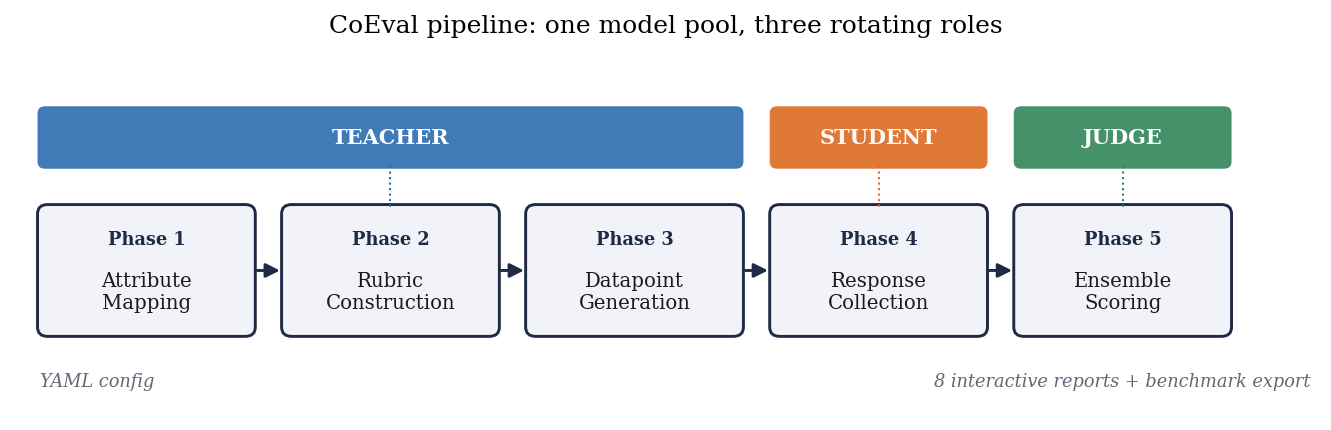
\includegraphics[width=\textwidth]{figures/f1_architecture.png}
\caption{\textbf{Figure 4.} The CoEval pipeline. A single pool of models rotates through three roles:
teachers map attributes, construct rubrics, and generate fresh benchmark items (Phases~1--3); students
produce candidate responses (Phase~4); and a cross-family judge ensemble scores them (Phase~5). The entire
run is specified in one declarative configuration.}
\end{figure*}

\begin{table*}[t]
\centering
\small\setlength{\tabcolsep}{4pt}%
\caption{\textbf{Table F1.} Experimental configurations. Judge panels differ by experiment: the
ground-truth anchor (Section~5.1) uses a frontier cross-family panel; the reliability and bias studies
(Section~5.2, Appendix~E) use a deliberately heterogeneous panel that includes weak open-weight judges;
and the verticals (Section~5.4, Appendix~D) reuse one fixed cross-family panel. All students are
gpt-4o-mini, gpt-3.5-turbo, and llama-3.2-3b unless noted.}
\setlength{\tabcolsep}{4pt}
\begin{tabularx}{\textwidth}{>{\hsize=0.920\hsize\raggedright\arraybackslash}X >{\hsize=1.067\hsize\raggedright\arraybackslash}X >{\hsize=1.272\hsize\raggedright\arraybackslash}X >{\hsize=0.742\hsize\raggedright\arraybackslash}X}
\toprule
Experiment & Task(s) & Judge panel & Size \\
\midrule
5.1 ground truth & SciQ, ARC (exact-match QA) & gpt-4o, claude-sonnet-4, gemini-2.5-flash & 191 items / 573 resp. \\
5.2 reliability (5.1 summ. anchor) & code (BLEU), news + text summ. (BERTScore) & gpt-4o-mini, gpt-3.5-turbo, claude-haiku, gemini-flash & 3 tasks / 900 resp. \\
5.2 + App.~E, App.~B & 4-task medium study & gpt-4o-mini, gpt-3.5-turbo, qwen2.5-1.5b, smollm2-1.7b & 7,978 eval. \\
5.4 verticals & drug-interaction, clinical, legal & claude-haiku, gemini-flash, gpt-4o-mini & 40 items each \\
5.3 contamination & SciQ memorization & exact-match (no LLM judge) & 200 memorized / 100 fresh \\
\bottomrule
\end{tabularx}
\end{table*}

\section{Domain case studies (full results)}\label{appG}

The preceding sections validate CoEval\textquotesingle s components where ground truth is available. We now exercise the complete tool
in its intended regime on three custom verticals, \emph{drug--drug interaction reasoning}, \emph{clinical
reasoning}, and \emph{legal analysis}, for which we assume no task-specific labeled data and no trustworthy
public benchmark. The drug-interaction vertical is the sharpest case for the framework\textquotesingle s premise: a well-known public
benchmark exists (DDIExtraction-2013) but is a relation-\emph{extraction} corpus rather than clinical-decision
reasoning, and is old and freely available enough to be presumed present in pretraining, while the few clinically
realistic DDI-reasoning sets are private and number only in the hundreds of items. From a one-line description per
vertical, CoEval\textquotesingle s teacher generated 40 attribute-stratified items (for drug interactions, stratified over severity,
mechanism, and patient context), three candidate models answered them, and the cross-family ensemble
(OpenAI~+~Anthropic~+~Google) scored every response, all from a single configuration file, with
no human labels or raters. \hyperref[appC]{Appendix~C} shows the actual generated artifacts for all three
domains: the one-line seed, the auto-generated attribute strata and rubric, and a representative synthesized item.

On the drug-interaction vertical CoEval produces a \textbf{clean, fully unanimous ranking}: all three
cross-family judges agree on the complete order \texttt{gpt-4o-mini}~(\(0.770\)) \(>\) \texttt{gpt-3.5-turbo}
~(\(0.682\)) \(>\) \texttt{llama-3.2-3b}~(\(0.497\)), with non-overlapping confidence intervals separating every
model (Table~G1). The clinical and legal verticals are consistent: the ensemble ranks the smallest model weakest in
both, unanimously in clinical and two-of-three in legal (where the Anthropic judge ranks \texttt{gpt-3.5-turbo}
lowest): genuine disagreement a single judge would hide and a diverse ensemble surfaces; on clinical the two
stronger models are statistically close, which the overlapping intervals correctly expose. This is the operation the
framework is built for: producing a defensible model ranking for a bespoke domain in which a standard benchmark is
unavailable or untrustworthy.

A ranking is only possible if the items \emph{separate} the models, the generation-side analog of judge
discrimination: a good teacher writes questions on which candidates actually differ. We measure per-item
discriminativeness as the spread of candidate-model ensemble scores. Across the \(120\) generated vertical items,
\textbf{\(71\%\) are discriminative} (a score range \(\ge 0.15\) across the three models), with a mean per-item
range of \(0.33\); on drug-interaction and legal analysis the figure rises to \(78\%\) and \(85\%\). Where the items do not
separate the models they are honest about it: clinical reasoning is only \(50\%\) discriminative precisely because its
two stronger candidates are genuinely close (\(0.873\) vs \(0.864\)), so the items reflect a real near-tie rather than
manufacturing a gap. This is why the panel yields non-overlapping ranking intervals: the teacher supplies items that
carry ranking signal, and a non-discriminative benchmark, on which every model scores alike, could not separate the
candidates no matter how reliable the judges are.

\begin{table}[tbp]
\centering
\small\setlength{\tabcolsep}{4pt}%
\caption{\textbf{Table G1.} CoEval ranks three candidate models on three custom, contamination-free verticals
generated from a task description with no labeled data. Scores are the cross-family ensemble mean ({[}0, 1{]}) with 95\%
bootstrap CI over 40 generated items. \texttt{llama-\allowbreak{}3.2-\allowbreak{}3b} ranks weakest in every vertical; the three judges
agree unanimously on the full drug-interaction order, unanimously on the weakest clinical model, and two-of-three in legal.}
\setlength{\tabcolsep}{4pt}
\begin{tabularx}{\linewidth}{>{\hsize=1.128\hsize\raggedright\arraybackslash}X >{\hsize=0.780\hsize\raggedright\arraybackslash}X >{\hsize=1.092\hsize\raggedright\arraybackslash}X}
\toprule
Vertical & Model & CoEval score {[}95\% CI{]} \\
\midrule
\emph{Drug--drug interaction} & gpt-4o-mini & 0.770 {[}0.739, 0.800{]} \\
& gpt-3.5-turbo & 0.682 {[}0.646, 0.717{]} \\
& llama-3.2-3b & 0.497 {[}0.459, 0.532{]} \\
\emph{Clinical reasoning} & gpt-3.5-turbo & 0.873 {[}0.849, 0.895{]} \\
& gpt-4o-mini & 0.864 {[}0.840, 0.885{]} \\
& llama-3.2-3b & 0.814 {[}0.784, 0.844{]} \\
\emph{Legal analysis} & gpt-4o-mini & 0.982 {[}0.973, 0.991{]} \\
& gpt-3.5-turbo & 0.740 {[}0.709, 0.770{]} \\
& llama-3.2-3b & 0.709 {[}0.677, 0.744{]} \\
\bottomrule
\end{tabularx}
\end{table}
